\chapter{Обменная симметрия, спин и два знака минус}

\section{Заполнение оболочек и вопрос о спин--статистике}

Обзор модели оболочек начинается с двух свойств, связанных с электронами. Электрон имеет спин, равный одной второй, с двумя безразмерными проекциями спина
\begin{equation}
m_s=+\frac12,
\qquad
m_s=-\frac12,
\end{equation}
и электроны подчиняются принципу запрета Паули. Эти факты связаны, но это не одно и то же утверждение.

Выражение ``одно и то же состояние'' требует осторожности. Два электрона не могут занимать одно и то же полное одночастичное состояние. Тем не менее два электрона могут находиться на одной пространственной орбитали, если их спиновые состояния различны. В приближении независимых электронов для гелия оба электрона занимают низшую пространственную орбиталь, один со спином вверх, а другой со спином вниз. Точнее, альтернативы ``у первого спин вверх, а у второго вниз'' и ``у первого спин вниз, а у второго вверх'' принадлежат запутанному двухэлектронному спиновому состоянию.

Это лишь старое приближение модели оболочек. Оно пренебрегает взаимодействием между электронами и используется здесь из-за простоты счета. Для лития первые два электрона заполняют низшую пространственную орбиталь с противоположными спинами. Третий не может войти ни в одно из этих полных состояний и должен занять более высокую орбиталь.

Следующий шаг — знакомая диаграмма орбитального углового момента. Секторы с
\begin{equation}
\ell=0,\qquad \ell=1,\qquad \ell=2
\end{equation}
называются \(S\)-, \(P\)- и \(D\)-состояниями. Для фиксированного значения \(\ell\) имеется
\begin{equation}
2\ell+1
\end{equation}
орбитальных состояний, так что
\begin{equation}
\ell=0\Rightarrow 1,
\qquad
\ell=1\Rightarrow 3,
\qquad
\ell=2\Rightarrow 5.
\end{equation}
В кулоновской задаче имеются дополнительные вырождения: радиальные уровни из разных \(\ell\)-секторов могут иметь одну и ту же энергию. Для аргумента о заполнении оболочек следующая оболочка содержит одну \(S\)-орбиталь и три \(P\)-орбитали. Поэтому число пространственных состояний равно
\begin{equation}
1+3=4
\end{equation}
Спин удваивает это число:
\begin{equation}
2(1+3)=8.
\end{equation}

Эти восемь полных одноэлектронных состояний заполняются в простой последовательности от лития до неона. После замкнутой оболочки у натрия снова имеется один внешний электрон, и потому в этой грубой картине он похож на литий. Химия здесь не является целью. Смысл состоит в том, что полуцелый спин и запрет Паули проявляются совместно.

Фотоны дают контрастный пример. Они имеют целый спин и не подчиняются правилу запрета. Классической электромагнитной волне соответствует множество фотонов, занимающих одну и ту же моду. Бозоны могут накапливаться в общем состоянии, тогда как тождественные фермионы не могут более одного раза занимать одно и то же полное состояние. Вопрос в том, могло ли это сочетание быть иным: полуцелый спин без запрета или целый спин с запретом. В трех пространственных измерениях соотношение спин--статистика дает отрицательный ответ. Привычное утверждение требует оговорок в одном и двух пространственных измерениях, и здесь не предпринимается попытки доказать этот результат теории поля.

\begin{classroomqa}
\lecturetimestamp{00:11:48}
\audiencequestion{Существует ли максимальное число бозонных квантов, которые могут занимать одно состояние?}
\lecturerresponse{Нет. Для бозонов нет предела заполняемости, и они склонны накапливаться в одном и том же состоянии.}
\end{classroomqa}

\section{Многочастичные волновые функции}

К этой связи мы подойдем через два знака минус: один возникает при обмене, другой при вращении. Начнем с обмена и временно опустим спин.

Пусть \(x_i\) обозначает положение частицы \(i\). Нижний индекс — это метка частицы, а не декартова компонента; три пространственные координаты собраны в один символ \(x_i\). Базис положений для \(n\) частиц имеет вид
\begin{equation}
\lvert x_1,x_2,\ldots,x_n\rangle.
\end{equation}
Для абстрактного состояния \(\lvert\Psi\rangle\) координатная волновая функция равна
\begin{equation}
\psi(x_1,x_2,\ldots,x_n)
=
\langle x_1,x_2,\ldots,x_n\mid\Psi\rangle.
\end{equation}
Ее квадрат модуля,
\begin{equation}
\bigl\lvert\psi(x_1,x_2,\ldots,x_n)\bigr\rvert^2,
\end{equation}
есть совместная плотность вероятности обнаружить частицу \(1\) в точке \(x_1\), частицу \(2\) в точке \(x_2\) и так далее.

Теперь предположим, что частицы тождественны. Сначала вообразим, что один электрон окрашен в синий цвет, а другой — в красный. Тогда ``синий в \(x_1\), красный в \(x_2\)'' можно было бы отличить от ``синий в \(x_2\), красный в \(x_1\).'' У реальных электронов нет ни таких цветов, ни индивидуальных меток. Перестановка учетных меток не может создать новую физическую конфигурацию.

Глобальная фаза не изменяет вероятности и средние значения. Для состояния в определенном секторе обменной симметрии координатная волновая функция может поэтому удовлетворять соотношению
\begin{equation}
\psi(x_2,x_1)=\eta\,\psi(x_1,x_2),
\qquad
\lvert\eta\rvert=1.
\end{equation}
Двукратное применение того же обмена возвращает исходные аргументы и дает
\begin{equation}
\eta^2=1,
\end{equation}
поэтому возможны два собственных значения при обмене
\begin{equation}
\eta=+1
\qquad\hbox{or}\qquad
\eta=-1.
\end{equation}

\editorialnote{Алгебра двукратного обмена определяет возможные собственные значения только после того, как предполагается, что состояние обладает определенным поведением при обмене. Дальнейшее ограничение, согласно которому допустимые состояния частиц данного вида лежат в одном секторе обменной симметрии, является физическим правилом; оно не следует из одного лишь \(\eta^2=1\). Та же оговорка относится и к аргументу о запрете ниже: антисимметрия влечет запрет после выбора фермионного сектора, но сама по себе алгебра обмена этот сектор не выбирает.}

Для бозонов допустимые волновые функции симметричны,
\begin{equation}
\psi_B(x_1,x_2)=\psi_B(x_2,x_1),
\end{equation}
тогда как для фермионов они антисимметричны,
\begin{equation}
\psi_F(x_1,x_2)=-\psi_F(x_2,x_1).
\end{equation}
Знак минус незаметен, когда он умножает всё состояние, но он существен, когда амплитуды складываются. Именно так обменная симметрия приобретает наблюдаемые следствия.

\section{Произведения, суммы и запрет}

Рассмотрим сначала две частицы, помещенные на одну и ту же одночастичную орбиталь \(\psi_0\). Их произведение имеет вид
\begin{equation}
\psi_0(x_1)\psi_0(x_2).
\end{equation}
Перестановка координат частиц дает
\begin{equation}
\psi_0(x_2)\psi_0(x_1)
=
\psi_0(x_1)\psi_0(x_2).
\end{equation}
Значения волновой функции — это числа, а не операторы, поэтому множители коммутируют. Произведение для одного и того же состояния симметрично. Это допустимая бозонная форма, но она не может описывать два тождественных фермиона.

Теперь поместим частицы на разные одночастичные орбитали:
\begin{equation}
\psi_0(x_1)\psi_1(x_2).
\end{equation}
Обмен дает
\begin{equation}
\psi_0(x_2)\psi_1(x_1).
\end{equation}
Для различных функций произведение после обмена, вообще говоря, не совпадает ни с исходным выражением, ни с его отрицанием. Поэтому простое произведение не обладает ни одной из требуемых обменных симметрий. Это не запрещает одной частице занимать \(\psi_0\), а другой — \(\psi_1\). Это означает, что двухчастичное состояние должно объединять оба способа распределения.

Симметричная комбинация имеет вид
\begin{equation}
\psi_B^{(01)}(x_1,x_2)
\propto
\psi_0(x_1)\psi_1(x_2)
+
\psi_0(x_2)\psi_1(x_1),
\end{equation}
а антисимметричная комбинация имеет вид
\begin{equation}
\psi_F^{(01)}(x_1,x_2)
\propto
\psi_0(x_1)\psi_1(x_2)
-
\psi_0(x_2)\psi_1(x_1).
\end{equation}
Знаков пропорциональности достаточно, поскольку для аргумента об обмене нормировка не нужна. В обоих состояниях по одной частице находится на каждой орбитали; они различаются только тем, как объединены два неразличимых способа распределения.

Теперь положим, что орбитали совпадают. Бозонная комбинация превращается в
\begin{align}
\psi_B^{(00)}(x_1,x_2)
&\propto
\psi_0(x_1)\psi_0(x_2)
+
\psi_0(x_2)\psi_0(x_1)\\
&=
2\psi_0(x_1)\psi_0(x_2),
\end{align}
и она ненулевая. Фермионная комбинация дает
\begin{align}
\psi_F^{(00)}(x_1,x_2)
&\propto
\psi_0(x_1)\psi_0(x_2)
-
\psi_0(x_2)\psi_0(x_1)\\
&=0.
\end{align}
Из антисимметричного правила обмена следует запрет: не существует ненулевого антисимметричного состояния, в котором оба фермиона находятся в одном и том же одночастичном состоянии.

Для многочастичного состояния это правило применимо к любой транспозиции двух аргументов. Транспозиция оставляет бозонную волновую функцию неизменной и меняет знак фермионной. Повторение одной и той же транспозиции тривиально в обоих случаях. Удивительно то, что один обмен, хотя он и не изменяет никаких наблюдаемых меток частиц, меняет знак фермионного состояния.

\section{Спин в полной метке частицы}

Теперь спин можно вернуть с небольшим изменением. Одночастичная амплитуда зависит и от положения, и от дискретной спиновой метки,
\begin{equation}
\psi(x,\sigma),
\end{equation}
где \(\sigma=+1\) или \(-1\) обозначает выбранное значение \(\sigma_z\). Квадрат модуля есть совместная плотность вероятности для указанного положения и спиновой метки.

Для многих частиц волновая функция имеет вид
\begin{equation}
\psi(x_1,\sigma_1;\,x_2,\sigma_2;\,\ldots).
\end{equation}
При обмене переставляется всё, что относится к двум частицам, а не только их положения:
\begin{align}
\psi_B(x_1,\sigma_1;\,x_2,\sigma_2)
&=
+\psi_B(x_2,\sigma_2;\,x_1,\sigma_1),\\
\psi_F(x_1,\sigma_1;\,x_2,\sigma_2)
&=
-\psi_F(x_2,\sigma_2;\,x_1,\sigma_1).
\end{align}
Это и есть точная форма вступительного утверждения модели оболочек. Два электрона могут находиться на одной пространственной орбитали только тогда, когда их полные состояния, включая спин, различны.

\begin{classroomqa}
\lecturetimestamp{00:34:33}
\audiencequestion{Является ли обменная симметрия проявлением группы перестановок?}
\lecturerresponse{Да. Обмен частиц — это перестановка, а закон преобразования со знаком плюс или минус задает представление группы перестановок.}
\end{classroomqa}

\begin{classroomqa}
\lecturetimestamp{00:35:12}
\audiencequestion{Почему двухчастичная конструкция является произведением, а не суммой одночастичных волновых функций?}
\lecturerresponse{Сумма описывает одну частицу в суперпозиции. Произведение принадлежит двухчастичному пространству тензорного произведения и описывает по одной частице в каждом одночастичном состоянии.}
\end{classroomqa}

Обмен полных меток показан на доске ниже.\footnote{Порядок координатно--спиновых меток восстановлен по разборчивому кадру доски и окружающему объяснению с 00:33:43 по 00:34:25.}
\begin{figure}[htbp]
\centering
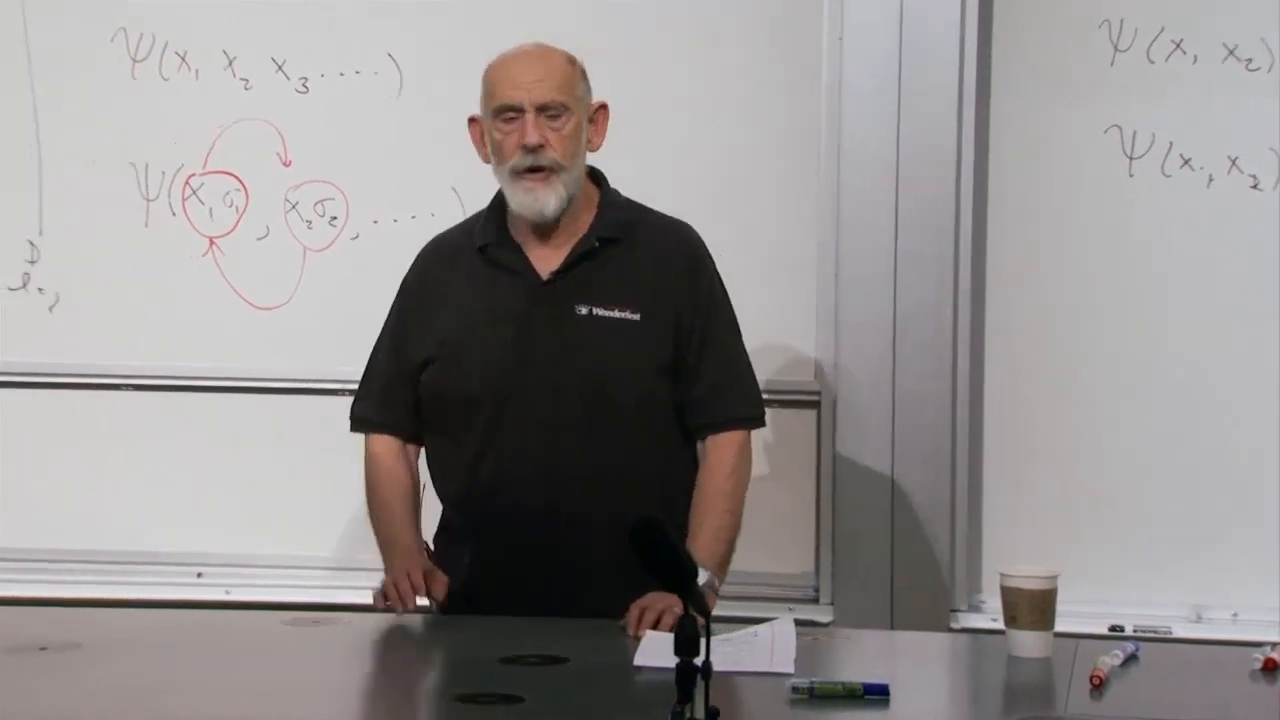
\includegraphics[width=0.9\linewidth]{lecture_05_frame_03.png}
\caption{При обмене двух тождественных частиц переставляются их полные координатно--спиновые метки. Бозонное состояние не меняется, тогда как фермионное меняет знак.}
\lectureframe{00:35:25}
\end{figure}

Это разные применения линейности. Для одной частицы
\begin{equation}
\alpha\psi_0(x)+\beta\psi_1(x)
\end{equation}
— это суперпозиция двух альтернатив. Для двух частиц
\begin{equation}
\psi_0(x_1)\psi_1(x_2)
\end{equation}
— это произведение, задающее амплитуду на пространстве с двумя координатами частиц. Симметризация или антисимметризация объединяет это произведение с соответствующим ему членом, полученным перестановкой частиц.

\begin{classroomqa}
\lecturetimestamp{00:36:13}
\audiencequestion{Порождает ли перестановка частиц интерференционный эффект?}
\lecturerresponse{Да. Исчезновение фермионной амплитуды для одного и того же состояния можно понять как деструктивную интерференцию между двумя вкладами, связанными перестановкой частиц.}
\end{classroomqa}

\begin{classroomqa}
\lecturetimestamp{00:37:13}
\audiencequestion{Вывел ли Паули правило запрета с помощью того же самого аргумента симметрии?}
\lecturerresponse{Паули исходил из эмпирического факта и нашёл математический формализм, в котором его можно было выразить. Поначалу он не выводил правило запрета из более фундаментальной теории.}
\end{classroomqa}

Антисимметрия даёт математический формализм, в котором выражается эмпирическое правило запрета.

\begin{classroomqa}
\lecturetimestamp{00:39:01}
\audiencequestion{Связана ли интерференция при перестановке частиц с интерференцией между альтернативными путями?}
\lecturerresponse{Да. В одной истории две частицы проходят, не пересекаясь, тогда как в другой они пересекаются и приходят в конечные точки друг друга. Для бозонов амплитуды складываются, а для фермионов могут взаимно уничтожаться.}
\end{classroomqa}

Перестановка даёт первый знак минус. Вращение даёт второй.

\section{Второй знак минус: вращение на \texorpdfstring{\(2\pi\)}{2 pi}}

Полный поворот, по-видимому, ничего не делает. Любое обычное геометрическое направление возвращается к исходному после угла \(2\pi\). Однако возвращаться обязаны вероятности и средние значения. Сам вектор состояния может вернуться с общей фазой, как и при перестановке.

\begin{classroomqa}
\lecturetimestamp{00:42:12}
\audiencequestion{Какая ось используется для вращения, и является ли генератором орбитальный момент импульса, спин или и то и другое?}
\lecturerresponse{Можно выбрать внешнюю ось; ниже в этом качестве берётся ось \(z\). Генератором служит полный момент импульса, включающий как орбитальный, так и спиновый вклады. Сам спин не обязан быть направлен вдоль выбранной оси.}
\end{classroomqa}

\editorialnote{В формулах для момента импульса в этом обсуждении используется \(\hbar=1\), поэтому \(m\) является безразмерным собственным значением \(J_z\).}

Пусть \(\psi(\theta)\) обозначает состояние, получаемое, когда параметр вращения проходит угол \(\theta\). В используемой здесь конвенции
\begin{equation}
J_z\psi(\theta)
=
-i\frac{\partial}{\partial\theta}\psi(\theta).
\end{equation}
Для состояния с определённым \(J_z\)
\begin{equation}
J_z\psi(\theta)=m\psi(\theta).
\end{equation}
Объединяя эти уравнения, получаем
\begin{equation}
-i\frac{\partial}{\partial\theta}\psi(\theta)
=
m\psi(\theta),
\end{equation}
с решением
\begin{equation}
\psi(\theta)=e^{im\theta}\psi(0).
\end{equation}

Допустимые значения \(m\) — целые или полуцелые. Поэтому
\begin{equation}
\psi(2\pi)
=
\begin{cases}
+\psi(0), & m\in\mathbb Z,\\[4pt]
-\psi(0), & m\in\mathbb Z+\tfrac12.
\end{cases}
\end{equation}
После ещё одного полного оборота
\begin{equation}
\psi(4\pi)=\psi(0)
\end{equation}
в обоих случаях. Это и есть второй знак минус: состояние из мультиплета с полуцелым моментом импульса меняет знак при вращении на \(2\pi\).

Знак не меняет \(\lvert\psi\rvert^2\), так что, когда он умножает всё состояние целиком, его не видно. Тем не менее вращение на \(2\pi\) не представляется тождественным оператором для состояния с полуцелым спином. Различие становится наблюдаемым, когда этот знак задаётся относительно другой когерентной амплитуды.

\section{Пути \texorpdfstring{\(2\pi\) и \(4\pi\)}{2 pi и 4 pi}}

Различие между \(2\pi\) и \(4\pi\) можно сделать наглядным без дальнейшей алгебры. Возьмите чашку в одну руку и поверните её на один полный оборот, не выпуская. Чашка возвращается к своей исходной ориентации, но рука оказывается перекрученной. Продолжите до второго полного оборота, и руку можно будет вернуть в исходное положение, не поворачивая чашку обратно.

В родственной конструкции сферу помещают внутрь коробки и соединяют её с коробкой нитями. Поворот сферы на \(2\pi\) оставляет нити спутанными. В обычном трёхмерном пространстве спутывание, связанное с поворотом на \(4\pi\), можно распутать. Существенна не просто конечная ориентация сферы, а путь, пройденный в пространстве вращений.

\begin{classroomqa}
\lecturetimestamp{00:54:22}
\audiencequestion{Если сферу дважды повернуть вокруг одной и той же оси, можно ли действительно распутать нити? Требует ли это ещё одного пространственного измерения?}
\lecturerresponse{Путь \(4\pi\) можно распутать в обычном трёхмерном пространстве. Время параметризует движение; это не ещё одно пространственное направление. Путь \(2\pi\) таким образом распутать нельзя, тогда как путь \(4\pi\) — можно.}
\end{classroomqa}

Эти демонстрации различают нетривиальный путь \(2\pi\) и распутываемый путь \(4\pi\), не развивая формальной теории группы вращений.

\section{Перестановка и вращение в представлении с ремнём}

Теперь два знака минус стоят рядом. Перестановка двух тождественных фермионов меняет знак их совместной волновой функции. Поворот состояния с полуцелым спином на \(2\pi\) тоже меняет его знак. Ремень даёт геометрическую связь между этими двумя операциями.

Расположите ремень так, чтобы два его нижних конца были переставлены местами. С другой точки зрения, тот же ремень несёт перекрут на \(2\pi\). Выполнение перестановки вместе с вращением на \(2\pi\) убирает перекрут и оставляет ремень без него. Комбинированный процесс можно непрерывно свести к тождественному преобразованию.\footnote{Наблюдение о перестановке--вращении в лекции приписывается David Finkelstein. В исходной записи не указана конкретная публикация, поэтому имя сохранено здесь только в качестве такой атрибуции.}

\begin{classroomqa}
\lecturetimestamp{01:01:12}
\audiencequestion{Не является ли это лишь утверждением о том, как ремень вложен в пространство, а не утверждением о топологии частиц?}
\lecturerresponse{Ремень можно интерпретировать как историю частиц в пространстве-времени. Если время направлено вверх, то поперечное сечение через него даёт частицеподобные объекты. Создаются пары, один объект поворачивается на \(2\pi\), и два тождественных объекта обмениваются местами. В этой истории фазы вращения и перестановки взаимно компенсируются.}
\end{classroomqa}

Эта история явно показывает учёт фаз. Начните с состояния без частиц. В двух разнесённых местах создайте пару частица--античастица, так что в промежуточный момент имеются четыре частицы. Поверните одну частицу на \(2\pi\), одновременно переставляя местами две тождественные частицы в другом месте конфигурации. Полную историю можно деформировать в элементарную историю, в которой пара создаётся, а затем аннигилирует. В обсуждаемом учёте знаков у этой тривиальной истории нет дополнительной фазы. Если \(\eta_{\mathrm{rot}}\) и \(\eta_{\mathrm{ex}}\) обозначают два этих знака, то описанную словами компенсацию можно кратко записать так\footnote{Это фазовое уравнение фиксирует компенсацию, описанную с 01:06:50 по 01:07:18; в лекции эта конструкция подаётся как наводящая на мысль, а не как строгое доказательство.}
\begin{equation}
\eta_{\mathrm{rot}}\eta_{\mathrm{ex}}=1.
\end{equation}

\begin{classroomqa}
\lecturetimestamp{01:03:34}
\audiencequestion{Можно ли связать перестановку с вращениями, повернув каждую из двух частиц на \(\pi\), а затем переориентировав их?}
\lecturerresponse{Эта конструкция может отражать родственную математику, но в ней используются два отдельных вращения на \(\pi\). Анализируемый здесь процесс содержит одно вращение на \(2\pi\), так что эти два аргумента не тождественны.}
\end{classroomqa}

Аргумент зависит от возможности создавать и аннигилировать частицеподобные объекты. В теории, чьи частицы были бы вечными, он не имел бы такой формы. Он также не предлагается как стандартное доказательство теоремы о спине--статистике. Его цель — показать топологическую причину того, почему знаки перестановки и вращения согласуются.

\section{Сгустки, зеркальные образы и аннигиляция}

Эту конструкцию можно повторить для локализованных конфигураций полей. Предположим, что одно или несколько полей почти всюду принимают свои вакуумные значения, но в малой области имеют ненулевые профиль и структуру. Такая локализованная конфигурация — сгусток.

Теперь постройте вторую конфигурацию как подходящий зеркальный образ первой. Одну назовите частицей, другую — античастицей. Сблизьте их. Соответствующие части конфигураций поля встречаются и взаимно гасят друг друга. На промежуточной стадии некоторые части сгустков, возможно, уже исчезли, тогда как другие ещё остаются. Продолжение деформации убирает оставшуюся структуру и возвращает поля к вакуумной конфигурации. Два противоположно направленных перекрута ремня дают ту же картину: сдвиньте их вместе, и они раскрутятся.

Этот процесс можно пустить в обратную сторону. Пустое пространство может породить сгусток и его зеркального партнёра. Можно создать две такие пары, повернуть один сгусток на \(2\pi\), переставить местами два тождественных сгустка и затем снова аннигилировать эти пары. Тогда действует та же компенсация перестановки--вращения. Это по-прежнему эвристическое расширение конструкции, а не теорема о каждом локализованном возбуждении.

\begin{classroomqa}
\lecturetimestamp{01:11:30}
\audiencequestion{Существуют ли физические реализации этих сгусткоподобных конфигураций поля?}
\lecturerresponse{Да. Примеры включают ядра в описаниях скирмионного типа, магнитные монополи и другие частицеподобные возбуждения полей.}
\end{classroomqa}

Именно картина зеркального сгустка делает это обобщение понятным. Существенно не то, что объект изначально был элементарной точечной частицей, а то, что частицеподобное возбуждение и его партнёр могут быть созданы, сближены и аннигилированы непрерывным образом. Это свойство и мотивирует более общее соотношение между поведением при вращении и при обмене.

\begin{classroomqa}
\lecturetimestamp{01:16:12}
\audiencequestion{Означает ли спин 1/2, что состояние накапливает только половину обычной фазы вращения?}
\lecturerresponse{Фаза в этом соглашении равна \(e^{im\theta}\). При полуцелом \(m\) поворот на \(2\pi\) даёт \(-1\), тогда как поворот на \(4\pi\) даёт \(+1\).}
\end{classroomqa}

\section{Глобальный знак и нулевой эксперимент}

Можно ли наблюдать минус-знак от поворота на \(2\pi\)? Начнём с эксперимента, в котором это невозможно. Удержите электрон в магнитном поле, дайте его спину следовать за полем, пока установка медленно поворачивается на \(2\pi\), а затем выпустите электрон в интерференционную установку. Сравните это с той же процедурой без поворота.

Поворот изменяет состояние следующим образом:
\begin{equation}
\psi\longmapsto-\psi,
\end{equation}
но минус-знак умножает всё состояние целиком. Все вероятности остаются неизменными, поэтому итоговая интерференционная картина не сохраняет никаких сведений о том, был ли предварительный поворот. Это нулевой эксперимент: общей фазе не с чем интерферировать.

\begin{classroomqa}
\lecturetimestamp{01:20:01}
\audiencequestion{Почему поворот магнитного поля нужно выполнять медленно?}
\lecturerresponse{Спин должен продолжать следовать за вращающимся магнитным полем. Если поле вращать слишком быстро, спин перестанет за ним следовать.}
\end{classroomqa}

\section{Один электрон в двух когерентных ветвях}

Знак становится наблюдаемым, когда его делают относительным. Пропустите один электрон через делитель пучка. Часть его волновой функции идёт по одному пути, а часть — по другому:
\begin{equation}
\psi(x)=\psi_1(x)+\psi_2(x).
\end{equation}
Это один электрон, а не два электрона. Он находится в когерентной суперпозиции двух альтернатив. Это различие нужно ясно сохранять: два пакета не являются двумя независимыми частицами.

Направьте два пакета в отдельные области, содержащие магнитные поля. Поверните поле в одной области на \(2\pi\), оставив поле в другой без изменения. Для состояния с полуцелым спином,
\begin{equation}
\psi_1(x)+\psi_2(x)
\longmapsto
\psi_1(x)-\psi_2(x),
\end{equation}
где метка повёрнутой ветви выбрана равной \(2\). Теперь знак является относительным. Когда позднее два пакета перекроются, сложение заменится вычитанием. Точка конструктивной интерференции может превратиться в точку деструктивной интерференции или даже в узел.

\begin{classroomqa}
\lecturetimestamp{01:23:46}
\audiencequestion{Что именно поворачивается, если есть только один электрон, но две ветви волновой функции?}
\lecturerresponse{Электрон находится в когерентной суперпозиции двух локализованных альтернатив. Одна ветвь поворачивается, а другая — нет. Если открыть ящики, чтобы узнать, какая из альтернатив реализовалась, это измерение разрушит интерференцию.}
\end{classroomqa}

Открытие ящиков обнаружило бы только один электрон — в одном ящике или в другом. Без этого измерения обе амплитуды остаются в состоянии. При повторении эксперимента интерференционная картина накапливается по одному событию детектирования за раз. В узле, созданном относительным минус-знаком, ни один электрон не детектируется.

\section{Магнитная прецессия и двухщелевая интерференция}

Более практичная схематическая постановка заменяет очень медленный эксперимент с ящиками. Разделите когерентную электронную волну на два пути. На одном пути пропустите электрон через магнитную область так, чтобы его спин сначала был поперечен полю. Затем спин прецессирует. Подбирая напряжённость поля и время пролёта, можно добиться, чтобы спин в этой ветви совершил один полный \(2\pi\)-оборот, тогда как другая ветвь не испытывает такого оборота.\footnote{В лекции сказано, что связанный с этим эксперимент со спинорной фазой был выполнен и что его принцип описан, но в исходной записи не указаны ни статья, ни конкретная установка. Поэтому изложение здесь ограничено конструкцией, данной в лекции.}

\begin{classroomqa}
\lecturetimestamp{01:27:05}
\audiencequestion{Как можно определить путь одиночного электрона?}
\lecturerresponse{Это нельзя определить, не испортив эксперимент. Любое измерение, регистрирующее, по какому пути прошёл электрон, разрушает интерференцию.}
\end{classroomqa}

\begin{classroomqa}
\lecturetimestamp{01:27:50}
\audiencequestion{Что именно представляет собой ветвь волновой функции и как делитель создаёт две ветви?}
\lecturerresponse{Ветвь — это волновой пакет, локализованный вдоль одного пути. Делитель превращает входящую волну в два пространственно разделённых пакета, а электрические или магнитные поля могут направлять эти пакеты по разным путям.}
\end{classroomqa}

Если не считать магнитной области, это двухщелевой эксперимент. Падающая электронная волна разделяется на два пакета. Выходящие волны расплываются в общую область детектирования, где их амплитуды перекрываются. При отсутствии относительного поворота центральные амплитуды могут складываться. Поворот спина на \(2\pi\) на одном из путей меняет знак одной амплитуды и может привести к взаимному сокращению тех же вкладов.

\begin{classroomqa}
\lecturetimestamp{01:30:46}
\audiencequestion{Как может возникать интерференция, если электрон проходит через разные трубки или щели?}
\lecturerresponse{Окончательное детектирование не выявляет путь. Две выходящие волновые амплитуды расплываются и перекрываются на детекторе. Попытка посмотреть, какой путь был пройден, разрушила бы интерференцию.}
\end{classroomqa}

\begin{classroomqa}
\lecturetimestamp{01:33:22}
\audiencequestion{Должен ли диаметр трубки или щели быть сравним с длиной волны электрона?}
\lecturerresponse{Для буквальной реализации двух щелей, основанной на дифракции, отверстие должно быть достаточно малым, чтобы вызвать нужное расплывание. Описываемая установка носит схематический характер, а не является практической конструкцией.}
\end{classroomqa}

\begin{classroomqa}
\lecturetimestamp{01:33:44}
\audiencequestion{Оставил бы соответствующий поворот поляризации фотонов на \(2\pi\) интерференционную картину неизменной?}
\lecturerresponse{Да. Фотоны имеют целый спин, поэтому полный поворот на \(2\pi\) не вводит фермионный минус-знак.}
\end{classroomqa}

\begin{classroomqa}
\lecturetimestamp{01:34:12}
\audiencequestion{В чём состоит небольшое отклонение практического эксперимента от идеализированной версии?}
\lecturerresponse{В идеальной конструкции спин поворачивается адиабатически. В практическом описании электрон проходит через магнитную область, и его спин прецессирует быстрее, но измеряемая фаза всё равно остаётся фазой, связанной с поворотом на \(2\pi\).}
\end{classroomqa}

Медленная схема выделяет саму идею, обеспечивая, что спин следует за полем без дополнительной динамики. Схема с прецессией динамически приводит к тому же относительному знаку. В любом варианте два пути должны перестать быть различимыми, прежде чем сможет появиться интерференционная картина.

\begin{classroomqa}
\lecturetimestamp{01:36:15}
\audiencequestion{Должны ли две ветви быть вновь объединены после делителя?}
\lecturerresponse{Да. Возникающие волновые пакеты должны перекрыться или расплыться в общую область детектирования, чтобы их амплитуды могли образовать интерференционную картину.}
\end{classroomqa}

\begin{classroomqa}
\lecturetimestamp{01:38:12}
\audiencequestion{Является ли этот эксперимент с поворотом одного электрона следствием принципа запрета Паули?}
\lecturerresponse{Нет. Здесь имеется только один электрон. Эксперимент измеряет спинорную фазу при вращении, а не запрет на нахождение двух фермионов в одном состоянии.}
\end{classroomqa}

\section{Интерференция при обмене и относительное вращение}

Обменный знак можно было бы выявить тем же общим методом, хотя предлагаемая установка сложнее. Начните с двух электронов и разделите их совместную волновую функцию на две когерентные ветви. Электронов по-прежнему только два, а не четыре: пара следует либо одной альтернативе, либо другой. Поменяйте два электрона местами в одной ветви, а в другой не обменивайте их. После того как ветви снова сведены вместе, фермионный знак обмена проявится как относительная фаза и может изменить интерференцию.

В последнем предложенном эксперименте два минус-знака сравниваются напрямую. Одна ветвь приобретает фермионную фазу обмена, тогда как другая приобретает соответствующую фазу вращения на \(2\pi\). Обе фазы равны \(-1\), так что относительный эффект компенсируется.\footnote{Запись между 01:40:26 и 01:41:15 ясно указывает на фазу обмена, фазу вращения на \(2\pi\) и их компенсацию, но точное приписывание вращения не удаётся восстановить по доступной записи речи.} В лекции это представлено как предлагаемый мысленный эксперимент, и сказано, что, насколько было известно лектору, он не был осуществлён.

\begin{classroomqa}
\lecturetimestamp{01:41:34}
\audiencequestion{Ставило бы наблюдение обменной фазы под вопрос неразличимость двух электронов?}
\lecturerresponse{Нет. Квантовая неразличимость тоньше, чем классическая тождественность. Она допускает, что вектор состояния меняет знак при обмене, хотя никакая наблюдаемая метка не различает частицы.}
\end{classroomqa}

Есть еще одна последняя оговорка. Поворот всего изолированного мира на \(2\pi\) дал бы лишь общую фазу, и никакой внутренний эксперимент не мог бы ее обнаружить. В обнаружимом эксперименте одна когерентная ветвь поворачивается относительно другой. Поэтому наблюдается не абсолютный знак, а интерференция, возникающая из-за относительного знака.
